\documentclass[letterpaper]{article}
\usepackage{geometry}
\geometry{margin=1.15in}
\usepackage[protrusion=true,expansion=true]{microtype}	
\usepackage[boxruled,linesnumbered,vlined,inoutnumbered]{algorithm2e}
\usepackage{amsmath}
\usepackage{amsthm}
\usepackage{amssymb}
\usepackage{mathtools}
\usepackage{mathrsfs}
\usepackage{soul}
\usepackage{natbib}
\usepackage{rotating}
\usepackage{gensymb}
\usepackage{lscape}
\usepackage{array}
\usepackage{makecell}
\renewcommand\theadalign{bc}
\renewcommand\theadfont{\bfseries}
\renewcommand\theadgape{\Gape[4pt]}
\renewcommand\cellgape{\Gape[4pt]}
\usepackage{courier}
\usepackage{lipsum}
\usepackage{graphicx}
\usepackage{subcaption}
\usepackage[space]{grffile}
\usepackage{xcolor}
\definecolor{light-grey}{rgb}{0.9,0.9,0.9}
\definecolor{dark-red}{rgb}{0.4,0.15,0.15}
\definecolor{dark-blue}{rgb}{0,0,0.7}
\usepackage{environ}
\setcounter{tocdepth}{2}
\renewcommand{\contentsname}{Table of Contents}
\usepackage{hyperref}
\hypersetup{
    colorlinks, linkcolor={dark-blue},
    citecolor={dark-blue}, urlcolor={dark-blue}
}

\setlength{\parskip}{1em}
\newcommand{\HIGHLIGHT}[1]{\textcolor{blue}{\textbf{#1}}}
\newcommand{\TODO}[1]{\textcolor{red}{\textbf{#1}}}

\begin{document}
%-----------------
%	Homework 2
%-----------------
\newpage
\begin{center}
    \begin{Large}
    COMPSCI 589 Homework 2 - Spring 2025
    \end{Large}
    \\
    \HIGHLIGHT{Due March 15, 2025, 11:59 pm Eastern Time}
\end{center}
\addcontentsline{toc}{subsection}{\textbf{Homework 2}}



\vspace{0.25in}
\section{Instructions}

\begin{itemize}
    \item This homework assignment consists of a programming portion. While you may discuss problems with your peers, you must answer the questions on your own and implement all solutions independently. In your submission, do explicitly list all students with whom you discussed this assignment. 
    \item We strongly recommend that you use \LaTeX~to prepare your submission. The assignment should be submitted on Gradescope as a PDF with marked answers via the Gradescope interface. The source code should be submitted via the Gradescope programming assignment as a .zip file. Include with your source code instructions for how to run your code. 
    \item We strongly encourage using Python 3 for your homework code. You may use other languages. In either case, you \textit{must} provide us with clear instructions on how to run your code and reproduce your experiments. 
    \item You may \textit{not} use any machine learning-specific libraries in your code, e.g., TensorFlow, PyTorch, or any machine learning algorithms implemented in scikit-learn (though you may use other functions provided by this library, such as one that splits a dataset into training and testing sets). You may use libraries like numpy and matplotlib. If you are not certain whether a specific library is allowed, do ask us.
    \item All submissions will be checked for plagiarism using two independent plagiarism-detection tools. Renaming variable or function names, moving code within a file, etc., are all strategies that \textit{do not} fool the plagiarism-detection tools we use. \textcolor{red}{If you get caught, all penalties mentioned in the syllabus \textit{will} be applied---which may include directly failing the course with a letter grade of ``F''}.
    \begin{center}
        \textcolor{red}{$\rightarrow$ Before starting this homework, please review this course's policies on plagiarism by  \\reading the corresponding section of the syllabus.}
    \end{center}
    
    \item The TeX file for this homework (which you should use in order to write your solutions in \LaTeX) can be found in the homework's .zip file on Canvas.

    \item The dataset we will investigate in this homework and the starting source code are available on Canvas. See below for more details.
    
\end{itemize}

\newpage

\vspace{1cm}
\section*{Programming Section (100 Points Total)}

In this homework, you will be implementing the Multinomial Naive Bayes algorithm. \textbf{Notice that you may \ul{not} use existing machine learning code for this problem: you must implement the learning algorithms entirely on your own and from scratch.} 
%
You will, in particular, train a Naive Bayes algorithm to classify Amazon reviews of CDs and vinyl as either positive or negative. The algorithm will be trained on the Amazon reviews dataset developed by Ni, Li, and McAuley (2019). 

\noindent Below, we first provide a brief review of the Multinomial Naive Bayes algorithm to help you revisit concepts covered in class, then discuss the structure of the dataset you will explore, and finally outline the experiments and analyses you should conduct.

\noindent \emph{\textbf{You can download the dataset and starting source code on Canvas.}}

\section{Multinomial Naive Bayes for Document Classification}

A Multinomial Naive Bayes model is trained based on a set of training \textit{documents}, each one belonging to a class. In this assignment, each document corresponds to one product review made by a user and posted on Amazon. You will be given a training set and a test set containing examples of positive product reviews and negative reviews. Recall that in the Multinomial Naive Bayes model, each document is represented by a Bag-of-Words vector $\mathbf{m}$ composed of integer entries; each entry in this vector indicates the frequency of a word in the document (see Fig.~\ref{fig:HW2_multinomial_repr.png} for an example).

    \begin{figure}[h!!!]
        \centering
        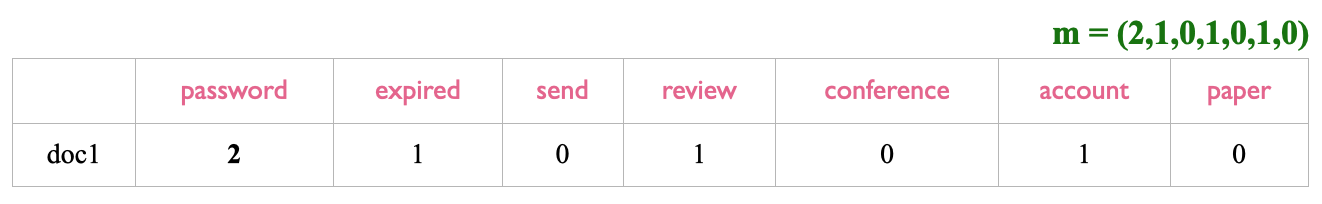
\includegraphics[width=0.85\textwidth]{figures/HW2_multinomial_repr.png}
        \caption{Example of how a document is represented by the Multinomial Naive Bayes algorithm.}
        \label{fig:HW2_multinomial_repr.png}
    \end{figure}

Assume a classification problem with $c$ classes. Let $y_i$ be the $i$-th class in the problem, where $1 \leq i \leq c$. Let \textbf{Doc} be a document, $len(Doc)$ be the number of \underline{unique} words appearing in \textbf{Doc}, and $w_k$ be the $k$-th unique word in the document, where $1 \leq k \leq len(Doc)$. Let $\Pr(y_i)$ be the prior probability of class $y_i$ and $\Pr(w_k \, | \, y_i)$ be the probability that word $w_k$ appears in documents of class $y_i$. Recall that when computing the latter probability, the Multinomial Naive Bayes model takes into account the \textit{frequency} with which the word appears in documents of that class, and not just \textit{whether} the word appears in documents of that class (as done, for example, by the Bernoulli Naive Bayes algorithm).

To classify a new document \textbf{Doc}, the algorithm computes, for each class $y_i$, the following probability:

\begin{equation}
    \Pr(y_i \, | \, \textbf{Doc}) \, = \, \Pr(y_i) \,\, \prod_{k=1}^{len(Doc)} \, \Pr(w_k \, | \, y_i).
    \label{eq:MNB}
\end{equation}

The algorithm then classifies \textbf{Doc} as belonging to the class that maximizes the probability in Eq.~\eqref{eq:MNB}.
%
To train the algorithm, one needs to estimate $\Pr(y_i)$, for each possible class, and $\Pr(w_k \, | \, y_i)$, for each possible word and class, given a training set. The prior probability of a class can be estimated, using examples from the training set, as follows:

\begin{equation}
\Pr(y_i) \, = \,\frac{N(y_i)}{N},
\end{equation}

\noindent where $N$ is the total number of documents available in the training set and $N(y_i)$ is the number of documents in the training set that belong to class $y_i$. Furthermore, the conditional probability of a word given a class can be estimated, using examples from the training set, as follows:

\begin{equation}
   \Pr(w_k \, | \, y_i) = \frac{n(w_k, y_i)}{\sum_{s=1}^{|V|} \, n(w_s, y_i)},
\end{equation}

\noindent where $n(w_k, y_i)$ is the frequency (total number of occurrences) of word $w_k$ in documents that belong to class $y_i$, $V$ is the vocabulary containing all unique words that appear in all documents of the training set, and $|V|$ is the length of the vocabulary.

\section{The CDs and Vinyl Amazon Reviews Dataset}

In this assignment, you will train a machine learning model to classify product reviews as positive or negative. Your algorithm will be trained on an Amazon reviews dataset. This dataset (which is provided to you on Canvas) is split into four files: ‘train-positive’, ‘train-negative’, ‘test-positive’, and ‘test-negative’, containing, respectively, positive and negative instances for training, and positive and negative instances for testing. To train the Multinomial Naive Bayes algorithm, each review/document first needs to be converted to a Bag-of-Words representation, similar to the one shown in Fig.~\ref{fig:HW2_multinomial_repr.png}. To do so, it is necessary to go through all the examples in the ‘train’ files (including both positive and negative reviews) and construct the vocabulary $V$ of all unique words that appear in the training set. Furthermore, each review that will be analyzed by your algorithm---either during the training process or when classifying new reviews---needs to be pre-processed: all words in the review should be converted to lowercase, stopwords (i.e., common words such as ``the'' and ``of'') should be removed from reviews, etc. We provide you with a function that performs such pre-processing tasks: \texttt{preprocess\_text()}, in the \texttt{utils.py} file. 

Since the dataset to be used in this assignment is relatively large, and you will have to conduct many experiments, we will not ask you to repeatedly manually split the dataset into training and test sets, conduct experiments many times, and evaluate the average performance. Instead, we provide you with one pre-computed split of the dataset; i.e., with one fixed training set and one fixed test set. Each of these sets contains 15,000 examples of positive reviews and 15,000 examples of negative reviews. This means that there is a total of 60,000 product reviews available, 30,000 of which will be used to train the Multinomial Naive Bayes algorithm, and 30,000 of which will be used to test it.

Furthermore, we also provide you with functions to load the product reviews (documents) that will be used as training and test sets: \texttt{load\_training\_set()} and \texttt{load\_test\_set()}, respectively. These functions can be found in the \texttt{utils.py} file. Both of them take as input two parameters: the percentage of positive and negative examples that should be randomly drawn from the training or test set, respectively. As an example, if you call \texttt{load\_training\_set(0.5, 0.3)}, the function will return a data structure containing approximately 50\% of the existing positive training examples, and approximately 30\% of the existing negative training examples. The function \texttt{load\_test\_set()} works similarly: calling \texttt{load\_test\_set(0.2, 0.1)} will return a data structure containing approximately 20\% of the existing positive test examples and approximately 10\% of the existing negative test examples. This capability is useful for two reasons: \textit{(i)} it allows you to work with very small datasets, at first, while you are still debugging your code, which makes it easier and faster to identify and solve problems; and \textit{(ii)} it will allow you, later, to quantify the impact that unbalanced datasets (i.e., datasets with significantly more examples of one of the classes) have on the performance of the model. You can find an example of how to use the above-mentioned functions in the file \texttt{run.py}, included as part of this assignment.

\subsection{Example}

Consider the following example. This is one of the 15,000 examples of a positive review included as part of the training set. Its contents are:

\noindent \texttt{This is a great CD with some old classics. I love listening while driving down the road. My kids don't hate it either.}

\noindent After pre-processing it (using the \texttt{preprocess\_text()} function) to remove punctuation, stopwords, etc., it becomes:

\noindent \texttt{great cd old classics love listening driving road kids dont hate either}

\noindent Assume, for simplicity, that the training set contains only two product reviews:

\noindent \textbf{(1)} \\
\noindent \texttt{Great box set by Wide Spread Panic. Song selection is good the recording was done top knotch. Very Good and I recommend it highly to those who are going to buy it.}

\noindent and

\noindent \textbf{(2)} \\
\noindent \texttt{I bought both the DVD and the CD.  The video is spellbinding and having the cd in my car is the perfect way to re-live the concert while I am traveling. I have replayed these so many times that I have memorized every note.  You can't wear this one out!}

In this case, the data structures returned by the function \texttt{load\_training\_set()} would look something like this:
\noindent \begin{verbatim}
[
  ['great', 'box', 'set', 'wide', 'spread', 'panic', 'song', 'selection', 
  'good', 'recording', 'done', 'top', 'knotch', 'good', 'recommend', 
  'highly', 'going', 'buy'],
  ['bought', 'dvd', 'cd', 'video', 'spellbinding', 'cd', 'car', 'perfect', 
  'way', 'live', 'concert', 'traveling', 'replayed', 'many', 'times', 
  'memorized', 'every', 'note', 'cant', 'wear', 'one']
]
\end{verbatim}

\noindent That is, a vector where each element corresponds to one of the reviews. Each element of the returned vector, in particular, is a Bag-of-Words vector containing the words that appear in the corresponding product review, after all pre-processing steps have been completed.


%--------------------------------------------


\section{Questions}

\textcolor{red}{\textbf{Hint}: While implementing and debugging your solution, we recommend loading only a small portion of the training and test sets. For example, calling the \texttt{load\_training\_set} and \texttt{load\_test\_set} functions with a parameter of 0.0004 will return approximately 0.04\% of each dataset—around 10 training and 10 test instances. This will make debugging significantly faster and easier.}



\noindent \HIGHLIGHT{Q.1 (18 Points)} You will first run an experiment to evaluate the performance of the standard Multinomial Naive Bayes algorithm. To do that, your implementation will---as discussed earlier---classify instances by computing posterior probabilities, $\Pr(y_i \, | \, Doc)$, according to the standard equation (Eq.~\eqref{eq:MNB}). In this experiment, you should use 20\% of the training set and 20\% of the test set; i.e., call the dataset-loading functions by passing $0.2$ as their parameters. First, classify all instances in the test set by comparing the posterior probabilities, $\Pr(y_i \, | \, Doc)$, for both classes. Then, report \textit{(i)} the accuracy of your model; \textit{(ii)} its precision; \textit{(iii)} its recall; and \textit{(iv)} the confusion matrix resulting from this experiment. 
%
% YOUR RESPONSE HERE
%



\noindent \HIGHLIGHT{Q.2 (18 Points)} One potential issue with the original Multinomial Naive Bayes formulation is that if a test instance contains a word that was not seen in training, then $\Pr(word|label)=0$. To mitigate this issue, one can employ \textit{Laplace Smoothing}. As discussed in class, this implies replacing the standard way of estimating the probability of a word $w_k$, given a class $y_i$, with the following equation:

\begin{equation}
    \Pr\left(w_k\,\,|\,\,y_i\right) = \frac{n(w_k, y_i) + 1}{\sum_{s=1}^{|V|} \, n(w_s, y_i) + |V|}.
\end{equation}

More generally, Laplace Smoothing can be performed according to a parametric equation, where instead of adding $1$ to the numerator, we adjust the probability of a word belonging to a class by adding a user-defined parameter $\alpha$ to the numerator, as follows:

\begin{equation}
    \Pr\left(w_k\,\,|\,\,y_i\right) = \frac{n(w_k, y_i) + \alpha}{\sum_{s=1}^{|V|} \, n(w_s, y_i) + \alpha |V|}.
\end{equation}

Intuitively, setting $\alpha = 0$ results in the standard formulation of Naive Bayes---which does not tackle the problem of words that do not appear in the training set. Suppose, alternatively, that we set $\alpha=4$. This is equivalent to adding 4 ``fake'' occurrences of that word to the training set, in order to avoid the zero-frequency problem. Using $\alpha=1000$, on the other hand, is equivalent to pretending we have seen that word 1000 times in the training set---even though we may have seen it, say, only 8 times. Although this solves the problem of zero-frequency words, it also strongly biases the model to ``believe'' that that word appears much more frequently than it actually does; and this could make the predictions made by the system less accurate. For these reasons, although it is important/necessary to perform Laplace Smoothing, we have to carefully pick the value of $\alpha$ that works best for our dataset. Using $\alpha=1$ is common, but other values might result in better performance, depending on the dataset being analyzed.


Another potential issue with the original Multinomial Naive Bayes formulation is that estimating the posterior probabilities using Eq.~\eqref{eq:MNB} can lead to numerical instability. This occurs, as discussed in class, because the computation involves multiplying hundreds or thousands of small terms, causing the probability estimate to rapidly approach zero. To tackle this issue, we often compare not $\Pr(y_1 \, | \, Doc)$ and $\Pr(y_2 \, | \, Doc)$, but the corresponding log-probabilities: $\log(\Pr(y_1 \, | \, Doc))$ and $\log(\Pr(y_2 \, | \, Doc))$. Taking the logarithm of such probabilities transforms the product of hundreds of terms into the sum of hundreds of terms---which avoids numerical issues. Importantly, it does not change which class is more likely according to the trained model. Concretely, when classifying a new instance, the log-probabilities that should be compared, for each class $y_i$, are as follows:

\begin{eqnarray}
    \log(\Pr(y_i \, | \, Doc)) \, &=& \, \log\left(\Pr(y_i) \,\, \prod_{k=1}^{len(Doc)} \, \Pr(w_k \, | \, y_i)\right) \\
    &=& \log(\Pr(y_i)) +\sum_{k=1}^{len(Doc)} \, \log(\Pr(w_k \, | \, y_i))  \label{eq:log_MNB}.
\end{eqnarray}

In this experiment, you should use 20\% of the training set and 20\% of the test set; i.e., call the dataset-loading functions by passing $0.2$ as their parameters. You should classify the instances in the test set by comparing log-probabilities, $\log(\Pr(y_i \, | \, Doc))$, according to Eq.~\eqref{eq:log_MNB}, for both classes. You should first report the confusion matrix, precision, recall, and accuracy of your classifier (when evaluated on the test set) when using $\alpha = 1$. Now, vary the value of $\alpha$ from 0.0001 to 1000, by multiplying $\alpha$ by 10 each time. That is, try values of $\alpha$ equal to 0.0001, 0.001, 0.01, 0.1, 1, 10, 100, and 1000. For each value, record the accuracy of the resulting model when evaluated on the test set. Then, create a plot of the model's accuracy on the test set (shown on the y-axis) as a function of the value of $\alpha$ (shown on the x-axis). The x-axis should represent $\alpha$ values and use a log scale. Analyze this graph and discuss why do you think the accuracy suffers when $\alpha$ is too high or too low.
%
% YOUR RESPONSE HERE
%




\noindent \HIGHLIGHT{Q.3 (18 Points)} Now you will investigate the impact of the training set size on the performance of the model. The classification of new instances, here, should be done by comparing the posterior log-probabilities, $\log(\Pr(y_i \, | \, Doc))$, according to Eq.~\eqref{eq:log_MNB}, for both classes. You should use the value of $\alpha$ that resulted in the highest accuracy according to your experiments in the previous question. In this question, you should use 100\% of the training set and 100\% of the test set; i.e., call the dataset-loading functions by passing $1.0$ as their parameters. Then, report \textit{(i)} the accuracy of your model; \textit{(ii)} its precision; \textit{(iii)} its recall; and \textit{(iv)} the confusion matrix resulting from this experiment.
%
% YOUR RESPONSE HERE
%



\noindent \HIGHLIGHT{Q.4 (18 Points)} Now repeat the experiment above but use only 30\% of the training instances; that is, load the training set by calling \texttt{load\_training\_set(0.3, 0.3)}. \textit{The entire test set should be used}. Report the same quantities as in the previous question. Discuss whether using such a smaller training set had any impact on the performance of your learned model. Analyze the confusion matrices (of this question and the previous one) and discuss whether one particular class was more affected by changing the size of the training set. 
%
% YOUR RESPONSE HERE
%




\noindent \HIGHLIGHT{Q.5 (10 Points)} In the document-classification application studied in this homework (i.e., one where ML is used to accurately classify product reviews), would you say that it is more important to have high accuracy, high precision, or high recall? Justify your opinion.
%
% YOUR RESPONSE HERE
%





\noindent \HIGHLIGHT{Q.6 (18 Points)} Finally, you will study how the performance of the learned model is affected by training it using an \textit{unbalanced} dataset (i.e., a dataset with significantly more examples of one of the classes). The classification of new instances, here, should be done by comparing the posterior log-probabilities, $\log(\Pr(y_i \, | \, Doc))$, according to Eq.~\eqref{eq:log_MNB}, for both classes. You should use the value of $\alpha$ that resulted in the highest accuracy according to your experiments in the previous questions. You will now conduct an experiment where you use only 10\% of the available \textit{positive} training instances and that uses  50\% of the available \textit{negative} training instances. That is, use \texttt{load\_training\_set(0.1, 0.5)}. \textit{The entire test set should be used}. Show the confusion matrix of your trained model, as well as its accuracy, precision, and recall. Compare this model's performance to the performance (according to these same metrics) of the model trained in question Q.4---that is, a model that was trained with a \textit{balanced} dataset. Discuss how training under an unbalanced dataset affected each of these performance metrics.
%
% YOUR RESPONSE HERE
%




\end{document}